\documentclass{VUMIFPSkursinis}
\usepackage{algorithmicx}
\usepackage{algorithm}
\usepackage{algpseudocode}
\usepackage{amsfonts}
\usepackage{amsmath}
\usepackage{bm}
\usepackage{caption}
\usepackage{color}
\usepackage{float}
\usepackage{graphicx}
\usepackage{listings}
\usepackage{subfig}
\usepackage{wrapfig}

% Titulinio aprašas
\university{Vilniaus universitetas}
\faculty{Matematikos ir informatikos fakultetas}
\institute{Informatikos institutas}  
\department{Programų sistemų studijų programa}
\papertype{Kursinis darbas}
\title{Vaizdo žaidimo eismo vaizdų generavimas naudojant nesuporuotų vaizdų transformacijas}
\titleineng{Video game traffic image generation using unpaired image to image translation}
\status{4 kurso 5 grupės studentas}
\author{Gytis Oksas}
\supervisor{j. asist. Boleslovas Dapkūnas}
\date{Vilnius – \the\year}

\setmainfont{Times New Roman}
\bibliography{bibliografija}

\begin{document}
\maketitle

\tableofcontents

\sectionnonum{Įvadas}
    Vaizdų transformacija (angl. \emph{image-to-image  translation}) yra plačiai taikoma metodika kompiuterių regos ir paveikslų apdorojimo problemoms spręsti \cite{ImTImTr}. Metodai, sprendžiantys šias problemas, gali būti taikomi parinktų specifinių paveikslėlių požymių keitimui, trūkstamų paveikslėlio pikselių užpildymui arba realistinių vaizdų generavimui. Ši taikymo sritis gali būti naudinga kuriant žaidimų meninį turinį (pavyzdžiui, tekstūras, realistinių objektų dizaino atitikmenis žaidimui), kuriant animacijas. Ir nors realių vaizdų transformavimas į nerealistinių vaizdų domeną nėra naujas (pavyzdžiui, veido nuotraukas transformuoti į animacinių filmukų stilių, kaip yra taikoma MSPC modelio pavyzdžiuose \cite{Mspc}), jis vis dar yra aktyviai analizuojamas, kadangi yra likusių ir pastoviai iškylančių problemų ir iššūkių (pavyzdžiui, vaizde daug triukšmo, besikartojantys artefaktai, nelogiški piešiniai). Vaizdo žaidimų vaizdų transformavimas į realistinius vaizdus yra spręstas, tačiau atvirkštinis variantas yra gan mažai išnagrinėtas.

    \begin{figure}[H]
        \centering
        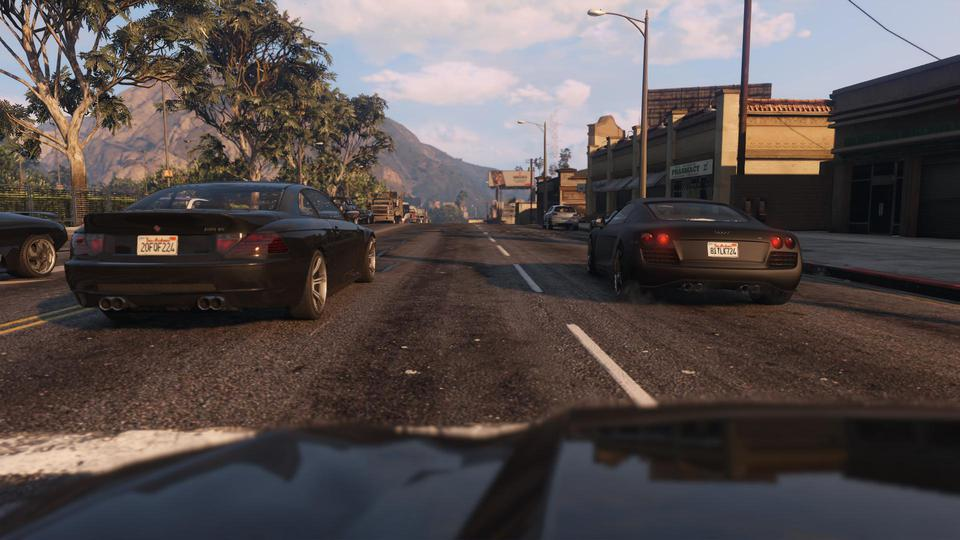
\includegraphics[scale=0.3]{img/EnPhEn_before}
        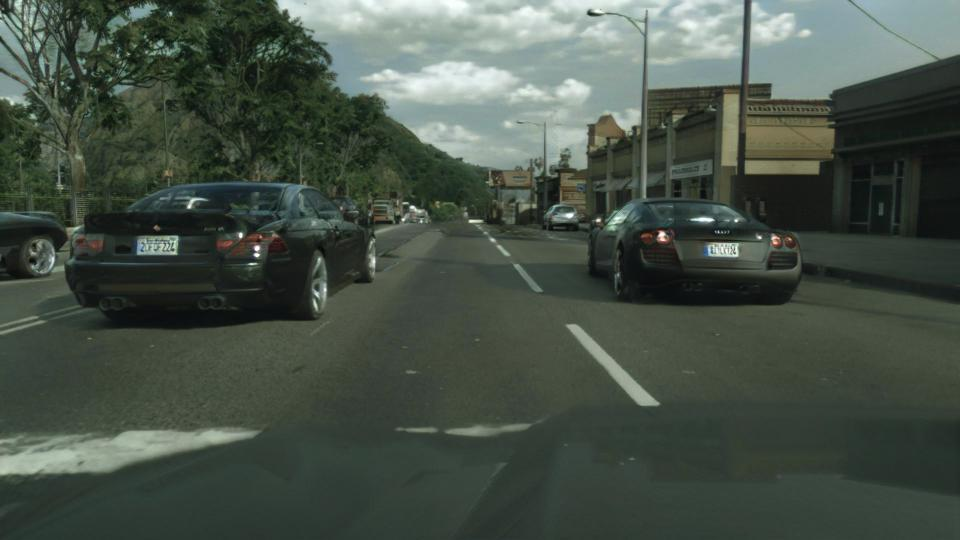
\includegraphics[scale=0.3]{img/EnPhEn_after}
        \caption{Vaizdai prieš ir po nuotraukos transformavimo, atitinkamai.\cite{EnPhEn}}
        \label{img:mlp}
    \end{figure}
    
    Tyrimas kuris atkreipė daug dirbtinio intelekto ir vaizdo žaidimų mėgėjų dėmesį yra aprašytas Intel dirbtinio intelekto mokslininkų straipsnyje „Enhancing Photorealism Enhancement“ \cite{EnPhEn}, jame pristatomas metodas, kaip išnaudojus modernias dirbtinio intelekto technologijas yra sukuriamas nuotraukų transformatoriaus modelis, sugebantis žaidimo GTA V automobilių eismo vaizdus paversti foto realistiniais, lyg įrašytais automobilio registratoriumi. Jis vienas pirmųjų įtikinamai, švariai, be prarastų esminių nuotraukų detalių ir be pridėtinių artefaktų sugebėjo transformuoti nuotrauką į realistiškai atrodantį vaizdą (žr. 1 pav.). Tai davė idėją šiam tyrimui – apsukti puses ir sukurti modelį, kuris pagal tuos pačius atributus sugebėtų transformuoti realybės automobilių eismo vaizdus į vaizdo žaidimo automobilių eismo vaizdus.
    
    Šio tyrimo tikslas ir yra sukurti modelį, kuris transformuotų nuotraukas iš realių į vaizdo žaidimų. Pasirinkta buvo transformuoti nuotraukas į  žaidimo „Grand Theft Auto: Vice City“ (toliau trumpinama „GTA:VC“) domeną dėl jo išskirtinio meninio stiliaus ir ryškaus domeno požymių skirtumo lyginant su realaus eismo nuotraukomis. Tyrimo uždaviniai:
    \begin{enumerate}
        \item Sukurti vaizdo žaidimo duomenų rinkinį.
        \item Apžvelgti modelius, tinkamus nesuporuotų vaizdų mokymui ir juos apmokyti.
        \item Palyginti modelius.
    \end{enumerate}
    
    
\section{Generatyviniai adversariniai tinklai}
    \subsection{GAN modelis}
        Pirmasis generatyvinis adversarinis tinklas (angl. \emph{generative adversarial network} – kontrastyvi neporuota transformacija) buvo pristatytas 2014 metais Montrealio universiteto mokslininkų \cite{OrigGan}. Jo principas sudarytas iš dviejų dalių. Pirmoji dalis yra generatyvinis modelis $G$, kuris išmoksta nuotraukų domeno požymius ir pagal juos sugeba kurti nuotraukas. Antroji – diskriminacinis modelis $D$, kurio tikslas yra gavus nuotrauką nuspėti tikimybę ar nuotrauka yra iš mokomo domeno, ar yra sugeneruota modelio $G$. Šiuo metodu, generatyvinis modelis $G$ yra pastoviai mokomas geriau kurti nuotraukas, kurios apgautų diskriminacinį modelį $D$, o diskriminacinis modelis $D$ yra pastoviai mokomas geriau atpažinti sugeneruotą nuotrauką nuo tikros.

        Šis modelis sugeba tik sukurti naujas nuotraukas, jų netransformuoja. Todėl jam reikia tik vieno duomenų rinkinio. Toliau šiame skyriuje minimi modeliai kuria nuotraukas jas transformuojant iš pirminės, todėl jiems reikalinga nuotraukos įvestis, jie taip pat reikalauja dviejų duomenų rinkinių – vieną šaltinio domeną ir vieną tikslo domeną.
    \subsection{CycleGAN modelis}
        Vienas iš trijų panaudotų nuotraukų transformavimo modelių yra CycleGAN modelis \cite{CycleGAN2017}. Šis modelis sukurtas 2017 metais ir išpopuliarėjo dėl savo galimybės vaizdus transformuoti į abi puses, t.y. modelį išmokius nuotraukas transformuoti iš domeno A į domeną B, jis taip pat sugebės vaizdus transformuoti iš domeno B į domeną A, nors nebūtinai taip pat gerai. Tai nulemia, jog modelį sudaro su generatyviniai modeliai ir du diskriminaciniai modeliai.

        Tyrimo straipsnyje yra vaizduojama, kaip modelis sugeba transformuoti vaizdus tarp realių domenų (pavyzdžiui, iš arklio į zebrą ir iš zebro į arklį) ir tarp ne nerealistinių ir realių (pavyzdžiui, iš kraštovaizdžio nuotraukų į Monet paveikslus ir atvirškčiai). Tarp dviejų nerealistinių domenų pavyzdžių nėra, tačiau galima nuspėti, jog su kokybišku apmokymo procesu ir duomenų rinkiniu tokį uždavinį taip pat nesunkiai įveiktų.

        Nors modelis jau lygintinai dirbtinio intelekto pasaulyje yra senas, tačiau dėl jo kodo realizacijos prieinamumo ir architektūros paprastumo yra vertas dėmesio ir laiko.
        
    \subsection{CUT modelis}
        Antras iš trijų naudotų modelių yra CUT (angl. \emph{contrastive unpaired translation} – kontrastyvi neporuota transformacija), išleistas 2020 metais. Pagrindinis jo bruožas yra, jog jis yra pritaikytas mokymui su nesuporuotomis nuotraukomis (t.y. nuotraukai iš domeno A, nėra tiesioginio atitikmens iš domeno B). Kitaip nei CycleGAN, CUT mokymas ir nuotraukų transformavimas vykdomas tik į vieną pusę, tai reiškia, kad norint nuotraukas transformuoti iš domeno A į domeną B ir iš domeno B į domeną A, yra reikalingi du atskirai išmokyti modeliai. Dėl vienpusio nuotraukų transformavimo, mokymo procedūra yra supaprastinama ir paspartinama. Šio modelio tikslas yra transformuojant perimti norimo domeno išvaizdą, bet išlaikyti transformuojamos nuotraukos struktūrą ir esminį turinį. Būtent ši CUT modelio savybė ir pakiša koją transformuojant nuotraukas kai kuriuose domenuose, kadangi jei apmokant modelį yra dažnai pasitaikančių artefaktų, tai jie gali dažnai atsikartoti ir transformuojamose nuotraukose, tai yra pabrėžiama „Enhancing Photorealism Enhancement“ \cite{EnPhEn} straipsnyje, kur transformuojant GTA V vaizdus, CUT modelis dažnai ant žaidėjo automobilio variklio dangčio uždėdavo Mercedes žvaigždę, kuri beveik visados matoma Cityscapes duomenų rinkinyje \cite{DaimCityDaSe}, kuriuo ir buvo mokinti modeliai.
    \subsection{MSPC modelis}
        Trečiasis naudotas modelis yra MSPC (angl. \emph{Maximum Spatial Perturbation Consistency} – maksimalus erdvinės perturbacijos pastovumas) \cite{Mspc}. Jis yra sukurtas CycleGAN \cite{CycleGAN2017} pagrindu, todėl jo nuotraukų transformavimas taip pat yra komutatyvus. Šis modelis yra sukurtas su tikslu jį naudoti nesuporuotų nuotraukų duomenų rinkiniams, kurie dažnai priveda prie nuotraukos turinio išdarkymo. Būtent šią problemą MSPC modelis ir bando spręsti, bandant geriau išsaugoti turinio bruožus ir jų turinį. Šis ir CycleGAN modeliai gali būtų mokomi suporuotais, nesuporuotais ir mišriais duomenų rinkiniais, tačiau sprendžiant šį uždavinį neįmanoma surinkti kokybiško ir kiekybiško suporuoto duomenų rinktinio, todėl yra parinktas šių modelių nesuporuoto mokymo metodas.
\section{Eksperimentas}
    Mokymo procesas vykdomas pagal keturis pagrindinius žingsnius: 
    \begin{enumerate}
        \item Duomenų rinkinio paruošimas,
        \item Modelių paruošimas;
        \item Mokymas;
        \item Rezultatų išvedimas.
    \end{enumerate}
    Jei rezultatai nėra patenkinami, tai ciklą kartojama nuo numanomo problemos taško. Šiame skyriuje aprašomi šio proceso žingsniai.
    \subsection{Duomenų rinkiniai}
            Vaizdų transformavimui iš realių į GTA:VC vaizdus reikia dviejų duomenų rinkinių: realaus eismo vaizdų ir žaidimo eismo vaizdų. Realaus eismo vaizdų duomenų rinkinių yra pakankamai daug, todėl jų rinkti nereikėjo ir buvo pasirinktas BDD100K\cite{BDD100K}  rinkinys, o GTA:VC vaizdams reikėjo kurti savo duomenų rinkinį, kadangi kokybiško ir kiekybiško rinkinio internete rasti nepavyko. 
        \subsubsection{Realių vaizdų duomenų rinkinys}
            Kaip minėta, buvo naudojamas BDD100K duomenų rinkinys. Jis sudarytas iš 100~000 automobilių eismo nuotraukų, padarytų naudojant kameras nukreiptas į automobilio važiavimo kryptį ir yra dažniausiai ant automobilio priekinės panelės. Buvo naudotas jo poaibis sudarytas iš 10~000 nuotraukų (dar vadinamas kaip bdd10k), kadangi GTA:VC nuotraukų duomenų rinkinys susidaro lygintinai mažas. 10 tūkst. nuotraukų duomenų rinkinys yra padalintas 70:20:10 santykiu mokymui, testavimui ir validacijai (atitinkamai gaunasi 7 tūkst, 2 tūkst ir 1 tūkst), nes kitaip rinkinys gautųsi stipriai nesubalansuotas. Kiekviena nuotrauka yra 1280:720 pikselių raiškos.
            
        \subsubsection{Grand Theft Auto: Vice City duomenų rinkinys}
            Eksperimentas buvo vykdomas su GTA:VC vaizdais, kurių duomenų rinkinį teko sukurti. Kokybišką duomenų rinkinį leidžia sukurti žaidimo grafiniai nustatymai, todėl papildomų modifikacijų į žaidimą diegti nereikia, užtenka ekrano vaizdo įrašymo programinės įrangos. Ekrano vaizdo įrašymui buvo naudojama OBS Studio programa.
            
            OBS Studio programos nustatyti parametrai, kad kuriamas duomenų rinkinys būtų struktūriškai kuo panašesnis į šaltinio duomenų rinkinį ir vaizdo įrašai nesigautų per dideli ir sunkiai apdorojami. Įgyvendinti du parametrų pakeitimai: įrašo raišką pakeista į BDD100K rinkinio nuotraukų raišką (kuri yra 1280:720 pikselių) ir nustatyta vieno kadro per sekundę įrašo sparta. Su paskutine parametru supaprastiname vaizdo įrašų perdarymą į nuotraukas, nes nereikia išmesti perteklinių nuotraukų nustačius didesnį kadrų dažnį (pvz. nustačius standartinius 60 kadrų per sekundę, gautume žymiai per daug nuotraukų).
            
            GTA:VC žaidimas reikalauja kelių vaizdinių pakeitimų tam, kad vaizdai būtų švaresni ir struktūriškai panašesni į BDD100K duomenų rinkinį. Naudojant standartinius nustatymus yra rodomas vaizdas trečiuoju asmeniu (t.y. iš žaidėjo galo), kuriame matyti daug interfeiso elementų (žr 2 pav.). Tam, kad vaizdas būtų artimesnis šaltinio domeno duomenų rinkiniui, reikėjo panaikinti žemėlapį ir informacines detales, tą žaidimas leido nustatymuose bei reikėjo nustatyti pirmą asmenį ir automobilio perspektyvos, kad nesimatytų pačio veikėjo ir taip išvengti nenorimų artefaktų (panašiai kaip įprastai lieka naudojant \cite{DaimCityDaSe} duomenų rinkinį, jame filmuojamas vaizdas iš automobilio Mercedes, o kadangi vaizduose yra matomas automobilio kapotas prie kurio pritvirtinta ikoniška Mercedes žvaigždė, todėl daugelyje transformuotų nuotraukų atsiranda minėtoji Mercedes žvaigždė). Šį pakeitimą žaidimas taip pat leidžia daryti, kaip konfiguracinį nustatymą. Šiuos pakeitimus implementavus, gaunamas kokybiškas ir švarus vaizdas, kuris nepalieka artefaktų ir užfiksuoja esminį turinį (žr. 3 pav.).

            \begin{figure}[H]
                \centering
                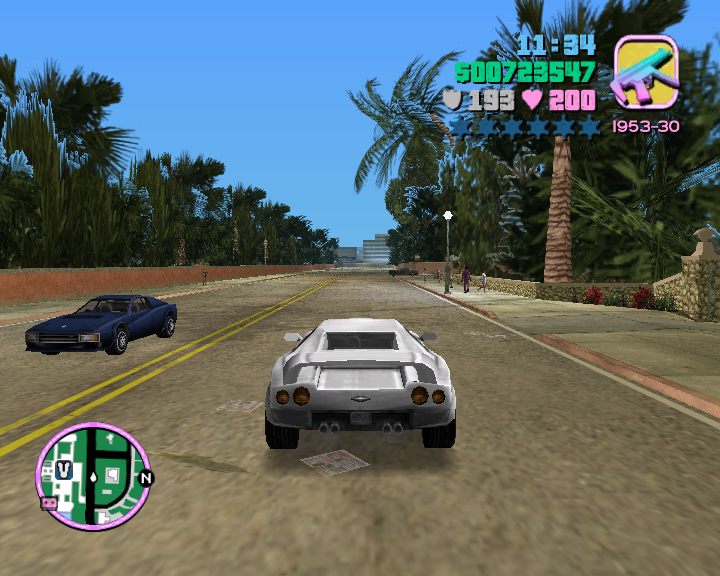
\includegraphics[scale=0.45]{img/neapdorotas_pvz}
                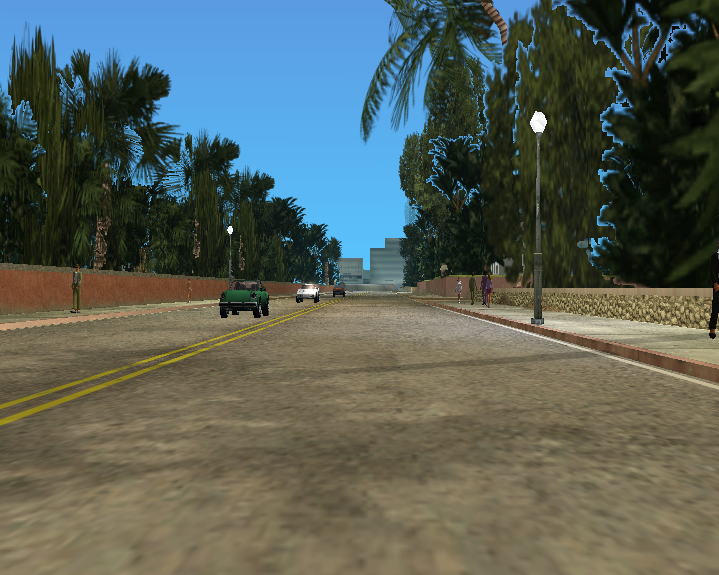
\includegraphics[scale=0.45]{img/apdorotas_pvz}
                \caption{GTA:VC žaidimo vaizdas su įprastais nustatymais (a) ir su pakeistais nustatymais (b).}
                \label{img:mlp}
            \end{figure}

            Duomenų rinkinio nuotraukos buvo kuriamos įrašinėjant GTA:VC žaidimo vaizdą, įrašuose važinėjant po žaidimo erdves keliais, bandant padengti kuo daugiau esamų vaizdų. Tas buvo daryta tiek žaidimo dienos metu, tiek nakties, kad būtų sukuriamas duomenų rinkinio aplinkybių vienodumas ir įvairumas. Žaidimo Pasaulis yra suskirstytas į 8 regionus. Kiekvieno regiono aplinka yra nufilmuojama žaidimo dienos ir nakties metu.
            
            Kitame skyriuje yra minima, jog rezultatuose yra pastebėta spragų – vaizdai turi žymiai mažiau automobilių nuotraukose nei BDD100K duomenų rinkinys, todėl po kelių eksperimentų, reikėjo papildyti surinktą duomenų rinkinį nuotraukomis, kuriuose yra daug automobilių arba jie užima didesnį ekrano plotą. Tokių nuotraukų iš viso buvo padaryta 300 ir jas pridėjus prie kitų nuotraukų buvo sukurta antra duomenų rinkinio versija.

            Vaizdo įrašai apdoroti Python kalbos skriptu, konvertuojančiu vaizdo įrašą į atskiras kadrų nuotraukas, taip sudarydamas GTA:VC vaizdų duomenų rinkinį sudarytą iš 2000 nuotraukų, o jo antrą versiją iš 2300.
        
        \subsection{Mokymo platformos}
            Paruošus modelius, jie buvo mokomi VU MIF superkompiuteriu. Mokoma buvo naudojant Linux Ubuntu operacinę sistemą (20.04 versiją) su PyTorch karkasu, pasitelkiant superkompiuterio Nvidia DGX-1 stotį, kurią sudaro keturios Nvidia Tesla V100 vaizdo plokštės.
        \subsection{Mokymo procesas} 
            Mokymui buvo išrinkti trys modeliai: CycleGAN\footnote{CycleGAN kodo realizacija pasiekiama nuoroda – \href{https://github.com/junyanz/pytorch-CycleGAN-and-pix2pix}}, CUT\footnote{CUT modelio kodo realizacija pasiekama nuoroda – \href{https://github.com/taesungp/contrastive-unpaired-translation}} ir MSPC\footnote{MSPC modelio kodo realizacija pasiekama nuoroda – \href{https://github.com/batmanlab/MSPC}}. Kadangi CUT ir MSPC kodo implementacija yra sukurta CycleGAN modelio realizacijos programinio kodo pagrindu, tiek duomenų rinkinio, tiek pačio mokymo proceso keisti drastiškai nereikėjo. 

            Kiekvienas modelis buvo mokomas 100 epochų su vientisu mokymo greičiu (0.0002) ir 35 epochomis tiesišku mokymosi greičio nykimu (angl. \emph{decay}).  Kiekvienas modelis buvo apmokytas du kartus, vieną kartą su pirmąja GTA:VC eismo vaizdų duomenų rinkiniu, o antrą kartą su antrąja jo versija, todėl iš viso yra kiekvieno modelio dvi versijos vadinamos V1 ir V2, pavyzdžiui, CUT V1 ir CUT V2. Mokymosi greitis yra apskaičiuojama pagal šią formulę:
            \[ lr = 2\times10^{-4} \times \frac{ max(0, ep - ep_n)}{ep_d + 1},\] čia $ep$ – einamoji epocha, $ep_{n}$ – epochų kiekis, $ep_{d}$ – nykimo epochų kiekis.

            CycleGAN ir MSPC modelių mokymas vyko žymiai ilgiau nei CUT modelio mokymo, dėl jų transformacijų komutatyvumo požymio, kadangi reikia nuotrauką transformuot tiek iš domeno A į B, tiek iš B į A ir MSPC modelio mokymas truko ilgiau nei CycleGAN dėl mažesnio skaičiavimų kiekio, reikalingų minėtam vaizdo detalių palaikymui.
            \begin{table}[H]\footnotesize
              \centering
              \caption{Modelių mokymo trukmės}
              {\begin{tabular}{|l|c|c|} \hline
                Modelio pavadinimas & Mokymo laikas, minutės\\
                \hline
                Cut V1 & 1524 \\
                Cut V2 & 1520 \\ 
                MSPC V1 & 4136 \\
                MSPC V2 & 3897 \\
                CycleGAN V1 & 2806 \\
                CycleGAN V2 & 2620 \\
                \hline
              \end{tabular}}
              \label{tab:table example}
            \end{table}

        \subsection{Modelių vertinimo metrika}
            Modelių nuotraukų transformavimo kokybei vertinti buvo parinkta FID (angl. \emph{Fréchet inception distance} – Fréchet pradžios atstumas) vertinimo metrika, dažnai naudojama vertinti modelių generuojamų nuotraukų kokybei. Šia metrika apskaičiuojamas atstumas tarp realių ir sugeneruotų nuotraukų požymių vektorių.

            Šis įvertis parodo, kaip nuotraukos iš dviejų grupių yra struktūriškai panašios. Žemesnis įvertis reiškia kokybiškesnes nuotraukas, o didelis – prastesnes. FID metrika pirmą kartą pristatyta ir panaudota 2017 metais Linco Johaneso Keplerio universiteto tyrimo straipsnyje pavadinimu „GANs Trained by a Two Time-Scale Update Rule Converge to a Local Nash Equilibrium“\cite{FidStart}. Šis įvertis pristatytas kaip geresnė metrika vietoj pradžios įverčio (angl. \emph{inception score}, trumpinama IS), kadangi IS vertina tik sugeneruotų nuotraukų kokybę, tačiau FID vertina sugeneruotų nuotraukų kokybę lyginant su šaltinio domeno duomenų rinkiniu.
            
        \subsection{„Dingstančių automobilių“ problema}
            Išmokius CycleGAN modelį buvo pastebėta, jog pradėjo dingti tam tikros stambios detalės iš nuotraukų, svarbiausia iš jų – automobiliai. Išmokyta pirmoji CycleGAN modelio versija linksta trinti automobilius ir uždengti tai aplinkos detalėmis ar fonu. Dėl to nuspręsta buvo išbandyti CUT modelį, kadangi jis pritaikytas nesuporuotų duomenų rinkinių uždaviniams, tačiau pirmoji jo versija yra dar labiau linkusi trinti automobilius iš nuotraukų. Dėl šios problemos taip pat buvo išbandytas MSPC modelis, nes juo yra sprendžiama nuotraukų semantinių detalių palaikymo problema. Nors MSPC modelis pasiekia geresnius rezultatus nei kiti du ties šia problema, tačiau išlaikomų automobilių kiekis vis tiek liko labai mažas (žr. 2 lentelę).
            \begin{figure}[H]
                \centering
                
\includegraphics[scale=0.8]{img/CycleGANV1/1_real_B}
                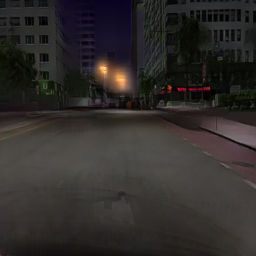
\includegraphics[scale=0.8]{img/CycleGANV1/1_fake_A}
                \captionsetup{width=.8\linewidth}
                \caption{CycleGAN modelio transformuotos nuotraukos pavyzdys, kuriame yra panaikinami automobiliai.}
                \label{img:mlp}
            \end{figure}
            \begin{table}[H]
                \footnotesize
                \centering
                \caption{Atpažintų automobilių kiekis duomenų rinkiniuose.}
                {\begin{tabular}{|l|c|c|} \hline
                    Modelio pavadinimas & Atpažintų automobilių kiekis, vnt. & Atpažintų automobilių dalis, \% \\
                    \hline
                    Testavimo duomenų rinkinys & 426 & - \\
                    CycleGAN V1 & 15 & 3,5 \% \\
                    CycleGAN V2 & 14 & 3,2 \% \\
                    Cut V1 & 7 & 1,6 \% \\
                    Cut V2 & 10 & 2,3 \% \\ 
                    MSPC V1 & 10 & 2,3 \% \\
                    MSPC V2 & 17 & 3,9 \% \\
                    \hline
                    \end{tabular}
                }
                \label{tab:table example}
            \end{table}
            Automobilių atpažinties nuotraukose testavimui naudojamas Centernet HG-104 \cite{CenterNet} modelis iš anksto apmokytas su Microsoft CoCo duomenų rinkiniu \cite{CocoDataset}. Šis modelis sugeba pakankamai gerai atpažinti automobilius net ir vaizdo žaidimuose kaip GTA:VC.
            
            Modeliai išmokyti su patobulintu duomenų rinkiniu, kuriame yra daugiau nuotraukų, kuriose yra automobilių užimančių pakankamai didelį nuotraukos plotą, arba yra nuotraukų su daug automobilių nuotraukoje, demonstruoja geresnį sugebėjimą išlaikyti automobilius (išskyrus su CycleGAN modeliu, kurio statistika minimaliai sumažėjo). Atpažintų automobilių padidėjimas siekia 69~\% su MSPC modeliu, tačiau toks patobulėjimas yra beveik bereikšmis kadangi bendras atpažintų automobilių procentas lieka labai mažas.
             
            Gali būti daug priežasčių, kodėl modeliai yra taip linkę trinti automobilius iš nuotraukų, tačiau labiausiai tikėtina iš jų yra automobilių kiekiai duomenų rinkiniuose – GTA:VC duomenų rinkinyje jų yra žymiai mažiau. 3 lentelėje yra pateikti mokymo duomenų rinkiniuose esantys automobilių kiekiai ir kokia dalis nuotraukų turi juose atpažintą bent vieną automobilį.
            \begin{table}[H]
                \footnotesize
                \centering
                \caption{Duomenų rinkinių atpažintų automobilių kiekiai ir nuotraukų.}
                {\begin{tabular}{|l|c|c|} \hline
                    Duomenų rinkinys & Atpažintų automobilių kiekis, vnt. & Dalis nuotraukų kuriuose yra atpažinta automobilių, \%\\
                    \hline
                    BDD100K & 21624 & 89 \%\\
                    GTA:VC V1 & 274 & 11 \%\\
                    GTA:VC V2 & 653 & 23 \%\\
                    \hline
                    \end{tabular}
                }
                \label{tab:table example}
            \end{table}

        \subsection{Paros meto keitimosi problema}
            Gautose nuotraukose pastebėta problema, jog tam tikrais atvejais yra pakeičiamas paros metas iš dienos į naktį. Tas dažniausiai įvyksta kai būna debesuota arba kai yra mažai matoma dangaus, tarkim kai aplinkui yra daug aukštų pastatų arba gamtos (žr. 5 pav.).
            \begin{figure}[H]
                \centering
                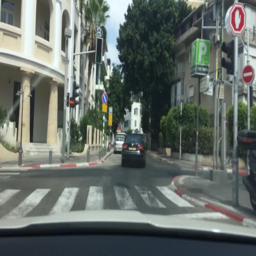
\includegraphics[scale=0.7]{img/aukstu_pastatu_real}
                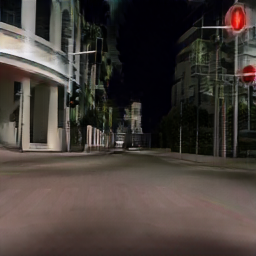
\includegraphics[scale=0.7]{img/aukstu_pastatu_fake}
                
\includegraphics[scale=0.7]{img/debesu_real}
                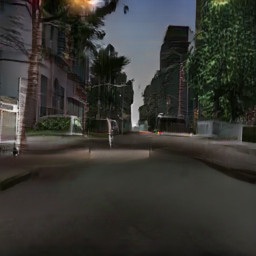
\includegraphics[scale=0.7]{img/debesu_fake}
                \caption{CycleGAN V2 pavyzdžiai kur modelio dėl aukštų pastatų arba debesų yra diena  pakeičiama į naktį.}
                \label{img:mlp}
            \end{figure}
        
        \subsection{Gauti FID įverčiai}
            Apmokius modelius buvo apskaičiuotos FID metrikos indikuojančios, kaip kokybiškai modeliai sugeba transformuoti nuotraukas lyginant su tikslo domenu.
            \begin{table}[H]
                \footnotesize
                \centering
                \caption{Apmokytų modelių gauti FID įverčiai ir atpažintų automobilių kiekiai.}
                {\begin{tabular}{|l|c|c|} \hline
                    Modelio pavadinimas & FID & Atpažintų automobilių kiekis, vnt.\\
                    \hline
                    CycleGAN V1 & 170 & 15\\
                    CycleGAN V2 & 167 & 14\\
                    Cut V1 & 181 & 7\\
                    Cut V2 & 186 & 10\\ 
                    MSPC V1 & 167 & 10\\
                    MSPC V2 & 145 & 17\\
                    \hline
                    \end{tabular}
                }
                \label{tab:table example}
            \end{table}

            Remiantis 4 lentelės duomenimis, matoma, jog geriausias FID nebūtinai reiškia geriausius rezultatus. Antroji apmokyta CycleGAN versija patobulino savo FID, tačiau, nors ir minimaliai, nukrito atpažįstamų automobilių skaičius, o CUT modeliui yra atvirkštinė situacija – antroji modelio versija padidino aptiktų automobilių skaičių, tačiau dėl to sumažėjo FID įvertis. Vienintelis modelis visiškai patobulėjęs nuo pagerinto GTA:VC duomenų rinkinio yra MSPC, jo atpažintų automobilių skaičius padidėjo ir FID įvertis sumažėjo. Pagal šiuos rezultatus matoma, jog iš trijų bandytų modelių, MSPC teikia geriausius rezultatus.
            
        \subsection*{Kokybiškai transformuojamos detalės}
            Modeliai itin gerai sugeba transformuoti gamtinius objektus, kaip žolė ir medžiai, iš realaus domeno į vaizdo žaidimo domeną. GTA:VC duomenų rinkinyje yra daug žaidime paplitusių palmių, kurios atrodo maždaug vienodai ir yra pavaizduotos 6 paveiksliuke.
            \begin{figure}[H]
                \centering
                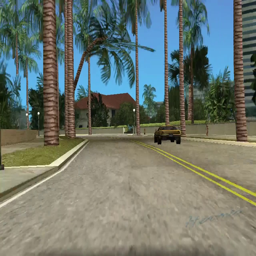
\includegraphics[scale=0.7]{img/palmiu_pvz}
                \caption{GTA:VC domeno palmių pavyzdys.}
                \label{img:mlp}
            \end{figure}
    
            Modelis medžius sugeba gerai atskirti ir juos transformuoti į GTA:VC domene matomus. Iš tamsiai žalios į šviesiai žalią spalvą pereinantys lapai yra nupiešiami medžiams ir net kamienai yra transformuojami į dryžuotai rudus. Ši elgsena yra būdinga visiems trims modeliams ir abejoms kiekvieno jų versijoms.
            \begin{figure}[H]
                \centering
                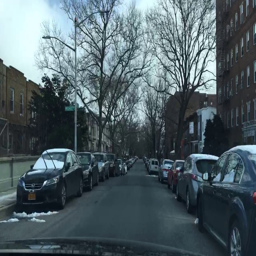
\includegraphics[scale=0.6]{img/palmiu_real}
                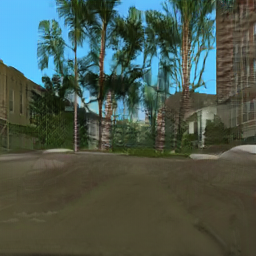
\includegraphics[scale=0.6]{img/palmiu_fake}
                \caption{MSPC V2 pavyzdžiai kur modelio dėl aukštų pastatų arba debesų yra diena  pakeičiama į naktį.}
                \label{img:mlp}
            \end{figure}
    
            Kitos dvi gerai transformuojamos detalės yra kelias ir dangus (kelio ir dangaus pavyzdys matomas 6 pav.). Dangus beveik visada įgauna įprastą saulėtos dienos mėlyną arba giedros nakties juodą spalvą. Nors, kaip prieš tai minėta, dangus kartais pakeičia dienos laiką, tačiau ir naktinis dangus yra tiksliai transformuojamas.
            Asfalto spalva taip pat yra labai gerai parenkama. Nors šios detalės yra labai paprastai transformuojamos, tačiau jos sudaro didelę dalį bendros transformuotos nuotraukos kokybės ir panašumo į vaizdo žaidimo domeną.
            
\sectionnonum{Rezultatai ir išvados}
    Gausesni transformuotų nuotraukų pavyzdžiai yra prisegti priedų skiltyje.
    
    Modelis pasiekęs žemiausią FID (145) yra MSPC V2. 
    
    Modelis, kurio transformuotuose vaizduose aptinkama daugiausia automobilių (3,9~\%) yra MSPC V2.
    
    Vaizdų transformavimas buvo įgyvendintas iki tokio lygio, kad galima nesunkiai atpažinti transformuoto vaizdo domeną, tačiau yra vietų, kurias tobulinti reikėtų, pagrindinė iš jų: nuotraukų semantinio turinio išlaikymas (paros metas, automobiliai). Modeliai dažnai panaikina automobilius iš transformuojamų nuotraukų, tačiau gerai sugeba transformuoti kelius, dangų ir gamtinius objektus.
    Tyrimo išvados:
    \begin{enumerate}
        \item Kokybiškiausius rezultatus duodantis modelis yra MSPC.
        \item Duomenų rinkinių struktūriniai ir objektų dažnumo skirtumai stipriai įtakoja nuotraukų transformavimo kokybę.
        \item Didesnis FID įvertis nebūtinai reiškia kokybiškesnį nuotraukos turinio išlaikymą.
    \end{enumerate}

\sectionnonum{Santrumpos}
    \begin{enumerate}
        \item \textbf{GTA:VC} – Žaidimas „Grand Theft Auto: Vice City“.
        \item \textbf{GTA V} – Žaidimas „Grand Theft Auto 5“.
        \item \textbf{FID} – angl. \emph{Fréchet inception distance} – Fréchet pradžios atstumas, yra metrika naudojama įvertinti generatyvinių modelių kokybę.
        \item \textbf{IS} – angl. \emph{Inception score} – pradžios įvertis, yra metrika naudojama įvertinti generatyvinių modelių kokybę.
    \end{enumerate}
    
        

\printbibliography[heading=bibintoc]

\appendix
    \section{Darbo saugykla}
        Darbo saugykla su duomenų rinkiniu, pavyzdinėmis nuotraukomis ir gautais modeliais yra pasiekiama nuoroda: \href{https://github.com/0ksas/kursinis}.

    \section{Nuotraukų pavyzdžiai (pirmosios duomenų rinkinio iteracijos)}
        \begin{table}[H]
            \footnotesize
            \centering
            \caption{Transformuojamų nuotraukų ir jų rezultatų pavyzdžiai}
            {\begin{tabular}{|c|c|c|c|} \hline
                Originali nuotrauka & CycleGAN  & CUT  & MSPC\\
                \hline
                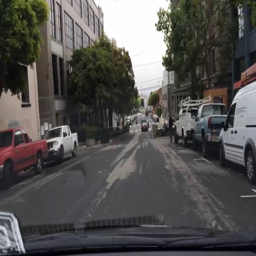
\includegraphics[scale=0.35]{img/pvz/1_real} & 
                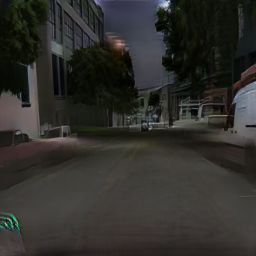
\includegraphics[scale=0.35]{img/pvz/1_cycle} & 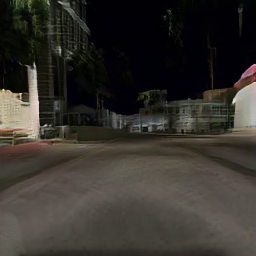
\includegraphics[scale=0.35]{img/pvz/1_cut} & 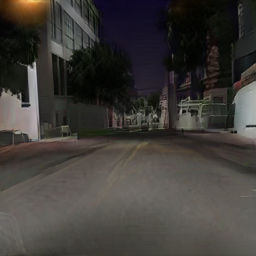
\includegraphics[scale=0.35]{img/pvz/1_mspc}
                \\
                \hline
                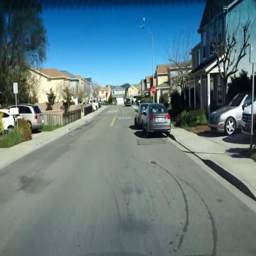
\includegraphics[scale=0.35]{img/pvz/3_real} & 
                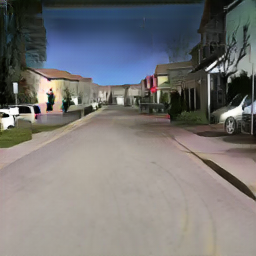
\includegraphics[scale=0.35]{img/pvz/3_cycle} & 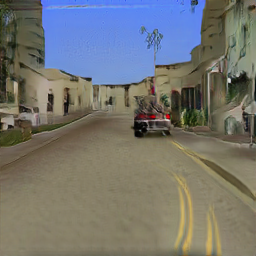
\includegraphics[scale=0.35]{img/pvz/3_cut} & 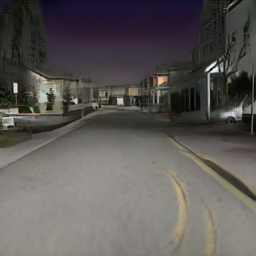
\includegraphics[scale=0.35]{img/pvz/3_mspc}
                \\
                \hline
                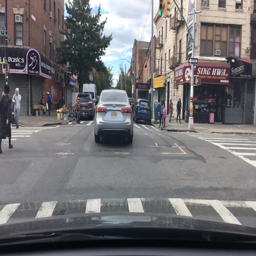
\includegraphics[scale=0.35]{img/pvz/4_real} & 
                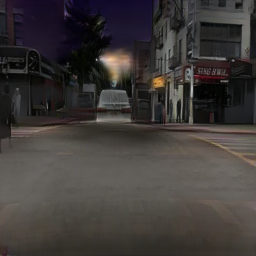
\includegraphics[scale=0.35]{img/pvz/4_cycle} & 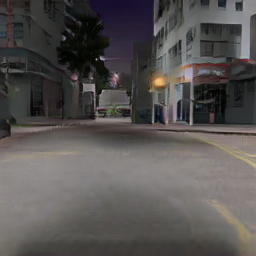
\includegraphics[scale=0.35]{img/pvz/4_cut} & 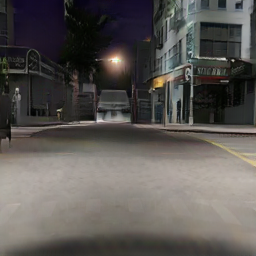
\includegraphics[scale=0.35]{img/pvz/4_mspc}
                \\
                \hline
                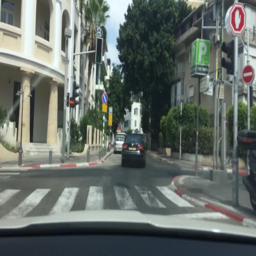
\includegraphics[scale=0.35]{img/pvz/5_real} & 
                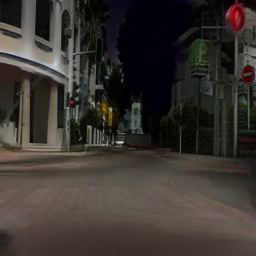
\includegraphics[scale=0.35]{img/pvz/5_cycle} & 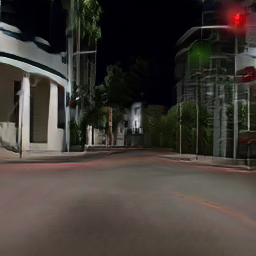
\includegraphics[scale=0.35]{img/pvz/5_cut} & 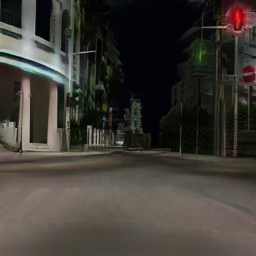
\includegraphics[scale=0.35]{img/pvz/5_mspc}
                \\
                \hline
                
\includegraphics[scale=0.35]{img/pvz/6_real} & 
                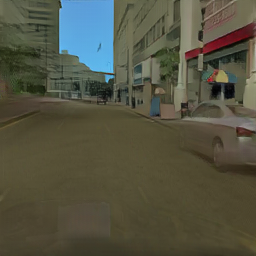
\includegraphics[scale=0.35]{img/pvz/6_cycle} & 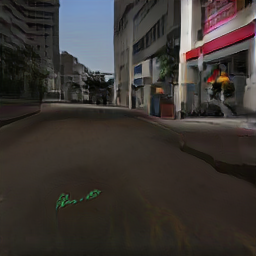
\includegraphics[scale=0.35]{img/pvz/6_cut} & 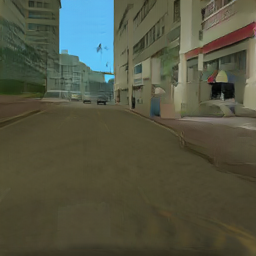
\includegraphics[scale=0.35]{img/pvz/6_mspc}
                \\
                \hline
                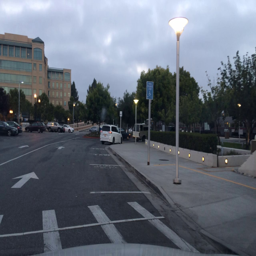
\includegraphics[scale=0.35]{img/pvz/7_real} & 
                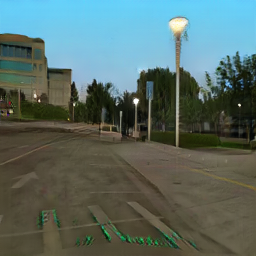
\includegraphics[scale=0.35]{img/pvz/7_cycle} & 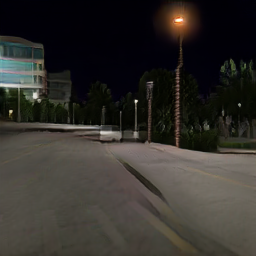
\includegraphics[scale=0.35]{img/pvz/7_cut} & 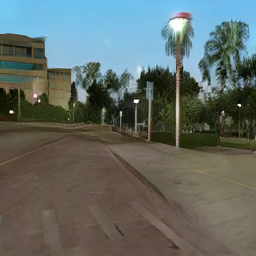
\includegraphics[scale=0.35]{img/pvz/7_mspc}
                \\
                \hline
                \end{tabular}
            }
            \label{tab:table example}
        \end{table}
    \section{Nuotraukų pavyzdžiai (antrosios duomenų rinkinio iteracijos)}
        \begin{table}[H]
            \footnotesize
            \centering
            \caption{Transformuojamų nuotraukų ir jų rezultatų pavyzdžiai}
            {\begin{tabular}{|c|c|c|c|} \hline
                Originali nuotrauka & CycleGAN V2  & CUT V2  & MSPC V2\\
                \hline
                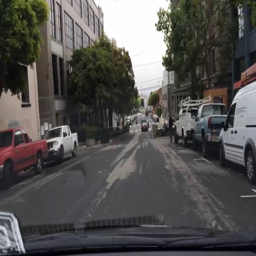
\includegraphics[scale=0.35]{img/pvz/1_real} & 
                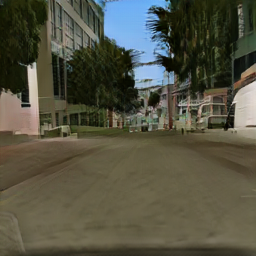
\includegraphics[scale=0.35]{img/pvz/1_cycle_v2} & 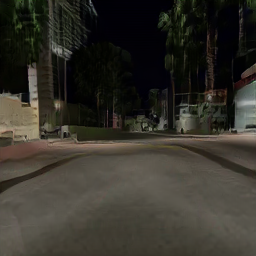
\includegraphics[scale=0.35]{img/pvz/1_cut_v2} & 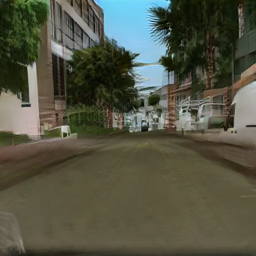
\includegraphics[scale=0.35]{img/pvz/1_mspc_v2}
                \\
                \hline
                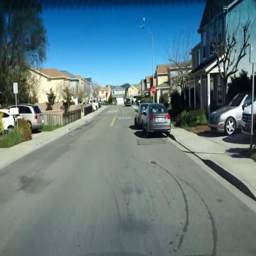
\includegraphics[scale=0.35]{img/pvz/3_real} & 
                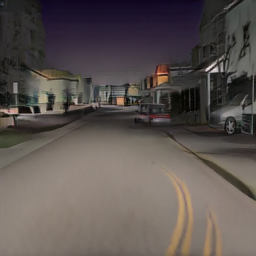
\includegraphics[scale=0.35]{img/pvz/3_cycle_v2} & 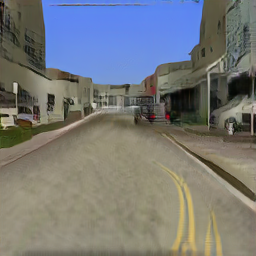
\includegraphics[scale=0.35]{img/pvz/3_cut_v2} & 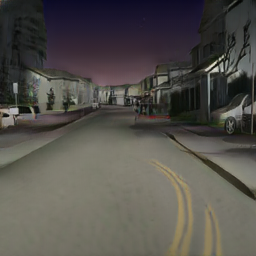
\includegraphics[scale=0.35]{img/pvz/3_mspc_v2}
                \\
                \hline
                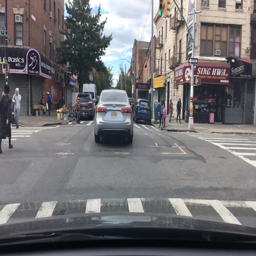
\includegraphics[scale=0.35]{img/pvz/4_real} & 
                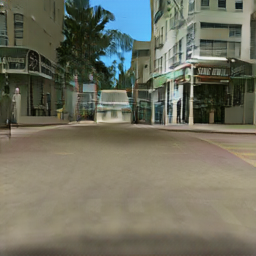
\includegraphics[scale=0.35]{img/pvz/4_cycle_v2} & 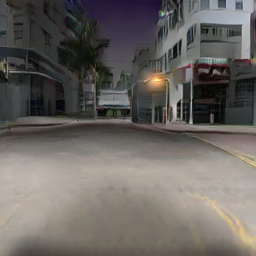
\includegraphics[scale=0.35]{img/pvz/4_cut_v2} & 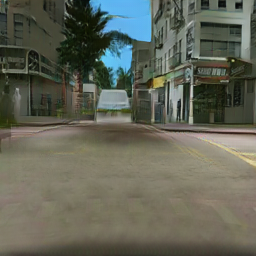
\includegraphics[scale=0.35]{img/pvz/4_mspc_v2}
                \\
                \hline
                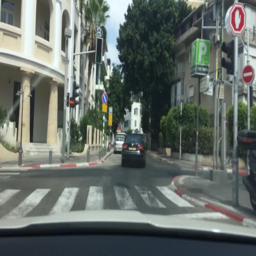
\includegraphics[scale=0.35]{img/pvz/5_real} & 
                \includegraphics[scale=0.35]{img/pvz/5_cycle_v2} & \includegraphics[scale=0.35]{img/pvz/5_cut_v2} & \includegraphics[scale=0.35]{img/pvz/5_mspc_v2}
                \\
                \hline
                \includegraphics[scale=0.35]{img/pvz/6_real} & 
                \includegraphics[scale=0.35]{img/pvz/6_cycle_v2} & \includegraphics[scale=0.35]{img/pvz/6_cut_v2} & \includegraphics[scale=0.35]{img/pvz/6_mspc_v2}
                \\
                \hline
                \includegraphics[scale=0.35]{img/pvz/7_real} & 
                \includegraphics[scale=0.35]{img/pvz/7_cycle_v2} & \includegraphics[scale=0.35]{img/pvz/7_cut_v2} & \includegraphics[scale=0.35]{img/pvz/7_mspc_v2}
                \\
                \hline
                \end{tabular}
            }
            \label{tab:table example}
        \end{table}
\end{document}
